\section{Durchführung}
\label{sec:Durchführung}
\subsection{Vorbereitung und Versuchsaufbau}
In der Versuchsvorbereitung wurden die Übergangs-Landé-Faktoren und die Energieaufspaltung der roten
$(^1\symup{P_1}\leftrightarrow {^1\symup{D_2}})$ und der blauen $(^3\symup{S_1}\leftrightarrow {^3\symup{P_1}})$ Linie einer
Cadmium-Lampe berechnet. Desweiteren wurden das Dispersionsgebiet für die verwendeten Wellenlängen sowie das
Auflösungsvermögen für die Lummer-Gehrcke Platte bestimmt.
Die Ergebnisse sind auf dem beigehefteten Blatt zu finden.\\
\\
In Abbildung \ref{fig:Aufbau} ist eine schematische Darstellung des Versuchsaufbaus zu finden.
\begin{figure}[H]
\center
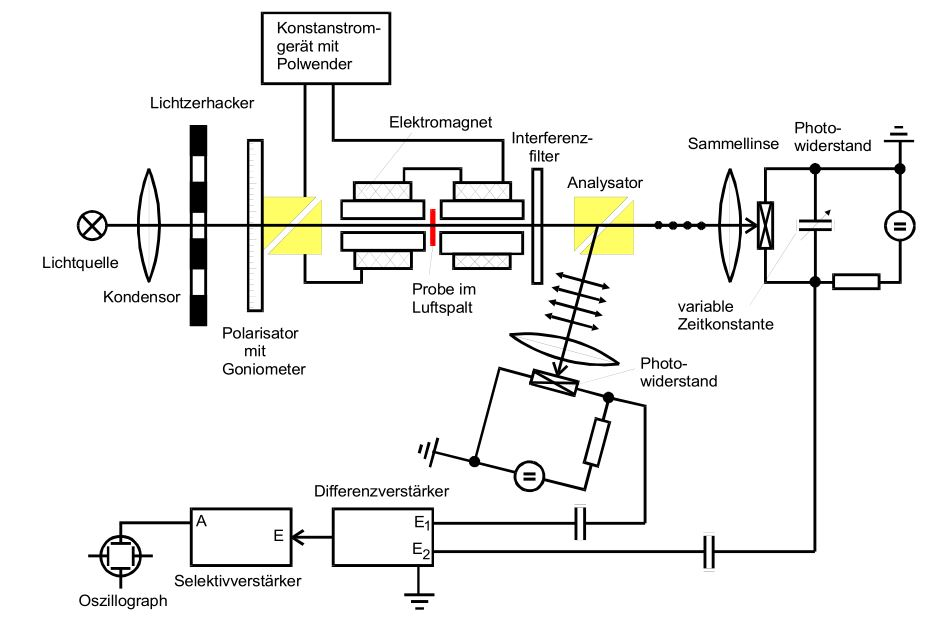
\includegraphics[width=0.8\textwidth]{pics/Aufbau.jpg}
\caption{Schematische Darstellung des Versuchsaufbaus \cite{Anleitung}.}  %?? ändern
\label{fig:Aufbau}
\end{figure}
Das für die Aufspaltung der Spektrallinien notwendige Magnetfeld wird von einem Elektromagneten erzeugt. Die
Cd-Lampe wird zwischen die Polschuhe des Magneten positioniert. Ein Objektiv bündelt das emmitierte Licht
zu Lichtstrahlen die durch eine Sammellinse und einen Spalt auf ein Geradsichtprisma gerichtet werden.
Dieses spaltet das Licht seiner Wellenlänge nach auf ohne die Richtung der optischen Achse zu ändern. Mit einem weiteren
Spalt wird die zu untersuchende Wellenlänge ausgewählt.
Desweiteren wird ein Polarisationsfilter eingebaut und mit weitern Linsensystemen wird das Licht auf
eine Lummer-Gehrcke-Platte abgebildet.
Innerhalb der Platte wird das Licht mehrfach reflektiert und die transmittierten Strahlen interfereieren mit
einander.
Ein beispielhafter Strahlengang in der Lummer-Gehrcke Platte ist in Abbildung \ref{fig:Gehrcke} zu erkennen.
\begin{figure}[H]
  \centering
  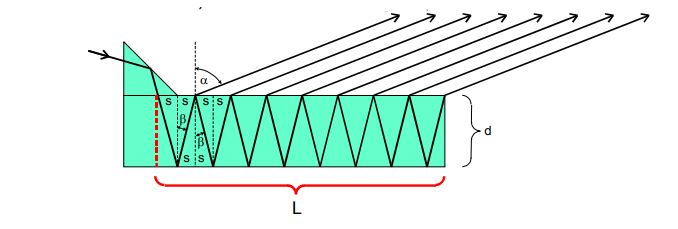
\includegraphics[width=0.7\textwidth]{pics/Lena-Gehrcke.JPG}
  \caption{Funktionsweise einer Lummer-Gehrcke Platte \cite{Anleitung}.}
  \label{fig:Gehrcke}
\end{figure}
Das sich bildene Interferenzmuster wird mit einer Digitalkamera aufgenommen.
\subsection{Versuchsdurchführung}
Zunächst wird mit einer Hallsonde das Magnetfeld ausgemessen. Dabei wird auf Hystereseeffekte geachtet und
sowohl der aufsteigende als auch der absteigende Ast für Stromstärken von 0 bis 20 A vermessen.\\
Dann werden die optischen Elemente justiert. Dabei wird mit der roten Linie ($\lambda = 643,8\,$nm)
begonnen. Der Polarationsfilter wird so eingestellt, dass der $\sigma$-Übergang beobachtet wird.\\
Wenn zwischen 10-15 Interfezlinien zu sehen sind wird zunächst ein Foto ohne Magnetfeld als Referenzbild gemacht.
Danach wird das Magnetfeld so lange erhöht bis eine eindeutige Aufspaltungzu sehen ist. Dabei ist darauf zu achten,
dass sich die neuen Linien nicht überlagern. Es wird wieder ein Bild aufgenommen. Auch wenn für die rote Linie
kein $\pi$-Übergang erwaret wird, da der normale Zeeman-Effekt auftritt, wird ein Bild gemacht.\\
\\Das selbe wird nun für die blaue Linie ($\lambda = 480,0\,$nm) wiederholt. Die Apperatur muss neu einjustiert werden
und es wird wieder ein Foto ohne Magnetfeld gemacht. Da bei dieser Wellenlänge der annormale Zeeman-Effekt auftritt, werden
bei eingeschaltetem Magnetfeld sowohl $\sigma$- als auch $\pi$-Übergänge erwartet und deswegen jeweils ein Foto mit
der 0° und 90° Einstellung des Polarisationsfilter gemacht.
